\documentclass[11pt, oneside]{article}   	% use "amsart" instead of "article" for AMSLaTeX format
\usepackage{geometry}                		% See geometry.pdf to learn the layout options. There are lots.
\geometry{letterpaper}                   		% ... or a4paper or a5paper or ... 
%\geometry{landscape}                		% Activate for for rotated page geometry
%\usepackage[parfill]{parskip}    		% Activate to begin paragraphs with an empty line rather than an indent
\usepackage{graphicx}				% Use pdf, png, jpg, or eps� with pdflatex; use eps in DVI mode
								% TeX will automatically convert eps --> pdf in pdflatex		
\usepackage{amssymb}
\usepackage{amsmath}
\usepackage{parskip}
\usepackage{color}
\usepackage{hyperref}

\title{Capacitor}
%\author{The Author}
%\section{}
%\subsection*{}
\date{}							% Activate to display a given date or no date

\graphicspath{{/Users/telliott_admin/Dropbox/Tex/png/}}
% \begin{center} 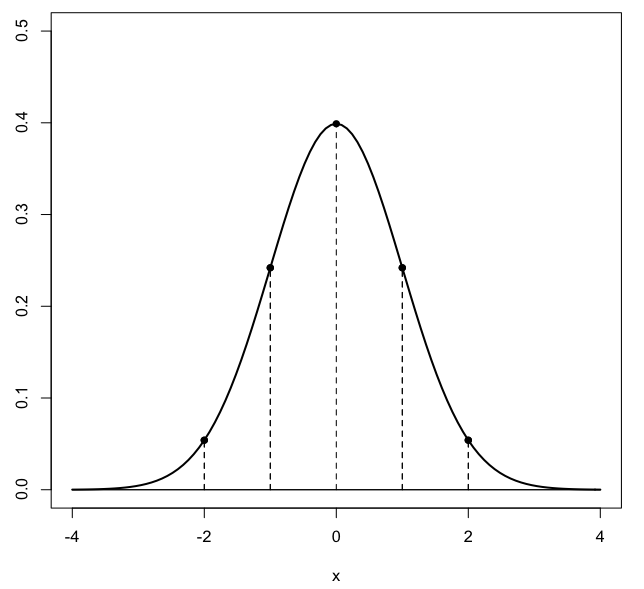
\includegraphics [scale=0.4] {gauss3.png} \end{center}
\begin{document}
\maketitle
\Large
A simple capacitor consists of two electrical conductors (metal plates, concentric spheres) separated by a dielectric (insulator).  A capacitor stores energy in the form of the electric field between the plates.

The potential difference is dependent on the amount of charge that is present, and physical characteristics like the size and geometry of the plates and the distance between them.

The capacitance is defined to be the ratio of the electric charge on each conductor to the potential difference
\[ C = \frac{Q}{V} \]
The unit is the farad, which is equal to one coulomb per volt.  Typical values might be microfarads $\mu F$.

A very useful property of capacitors is that they block direct current, yet allow alternating current to pass.  Also, when combined in appropriate circuits, they can be used to tune a circuit to a particular resonant frequency (e.g. in a radio).

The energy stored in a capacitor can be calculated as the work done in moving a small amount of charge "from" one plate "to" another.
\[ dW = V \ dq \]
\[ W = \int_0^Q V \ dq = \int_0^Q  \frac{q}{C} \ dq = \frac{1}{2} \frac{Q^2}{C}  \]
The integral here takes account of the fact that the voltage at the time any small charge $dq$ is transferred depends on how much charge is currently on the plates.

Since current does not actually flow across the capacitor, for each electron that leaves the positive plate, one must join the negative plate.  

Current is the time derivative of the charge
\[ i = \frac{dq}{dt} = \dot{q} \]

\[ \int i \ dt = \int dq = Q = VC \]
\[ V = \frac{1}{C} \int i \ dt \]
In a DC circuit with a voltage and a resistor
\[ V_0 = i(t)R + \frac{1}{C} \int_{t_0}^t i(t) dt \]
\[ \frac{d}{dt} \ V_0 = 0 = R \frac{di}{dt} +  i(t) \]
\[ RC\ \frac{di}{dt} + i = 0 \]
The rate of change of $i$ is proportional to $i$.  This is just an exponential with
\[ i(t) = i_0 e^{-t/RC} \]
\[ \frac{di}{dt} = -\frac{1}{RC} \ i_0 e^{-t/RC} \]
When you hook up a voltage and a capacitor, there is an initial current, but as the capacitor plates acquire charge the current dies away.

\subsection*{AC circuit}
If we put a capacitor into an AC circuit, then the charge is
\[ q(t) = CVe^{j\omega t} \]
where as before $C$ is a number that describes the capacity of the capacitor (with units of coulombs/volt), and $i$ is renamed to be $j$ because the electrical engineers use $i$ and $I$ for current.  Anyway the point is that the current across such a device is
\[ i(t) = \frac{dq}{dt} = j\omega CV e^{j\omega t} =  j\omega q(t) \]
To solve this differential equation, we need to find a function where
\[ i = \frac{dq}{dt} = j\omega q \]
If the voltage goes like the cosine, then this is a problem.

What we are going to do is to write the voltage as
\[ V(t) = V_o e^{j\omega t} \]
where $j = \sqrt{-1}$.  Then
\[ q(t) = C V_o e^{j\omega t}  \]
so the current is
\[ i(t) = j \omega C V_o e^{j\omega t}  \]
so the equivalent of the resistance for the capacitor is
\[ X_C = \frac{1}{j \omega C} \]
\[ = -\frac{j}{\omega C } \]
What does this mean?  It means that when the voltage is at the peak of its cycle, the current through the capacitor is 90 degrees out of phase with it.

\end{document}  